
\documentclass[letterpaper, 10 pt, conference]{ieeeconf}  % Comment this line out if you need a4paper



\IEEEoverridecommandlockouts                           

\overrideIEEEmargins                                   

\usepackage{graphicx}
\usepackage{caption}
\usepackage[cmex10]{amsmath}
\usepackage{algorithm}
\usepackage{algpseudocode}
\usepackage{enumerate}
\title{\LARGE \bf
Geometrical approach to On line Trajectory generation, Obstacle avoidance and Footstep planning for a Humanoid Robot
}

\author{ Kaustubh Nawade$^{1}$ V. Aditya$^{2}$ Apoorv Shrivastava$^{3}$ B. K. Rout$^{4}$% <-this % stops a space
%\thanks{The research project was funded by Dept. of Electronics and Information Technology, Govt. of India}
\thanks{$^{1}$B.E. (Hons.) Electrical \& Electronics \& M.Sc. (Hons.) Physics Undergraduate, BITS - Pilani
        {\tt\small kaustubh.nawade@gmail.com}}%
\thanks{$^{2}$B.E. (Hons.) Computer Science Undergraduate, BITS - Pilani
        {\tt\small 42vaditya@gmail.com}}%
\thanks{$^{3}$B.E. (Hons.) Mechanical, BITS - Pilani
        {\tt\small apoorvs92@gmail.com}}%
\thanks{$^{3}$Associate Professor, Dept. of Mech. Engg., BITS - Pilani
        {\tt\small rout@pilani.bits-pilani.ac.in}}%
}

\begin{document}



\maketitle
\thispagestyle{empty}
\pagestyle{empty}


%%%%%%%%%%%%%%%%%%%%%%%%%%%%%%%%%%%%%%%%%%%%%%%%%%%%%%%%%%%%%%%%%%%%%%%%%%%%%%%%
\begin{abstract}

This paper presents a unique real time technique for   path generation in dynamic environment using simple geometry, suitable for humanoid robots. We show that the proposed algorithm reduces computation to find the optimal collision free path by utilizing the geometrical shapes of the obstacles  to navigate from a known initial point to final point. The trajectory is then translated to known parameters of humanoid gait model thus effectively computing the footsteps for the robot. This algorithm has been simulated, implemented and tested on humanoid robot AcYut, developed at Centre for Robotics and Intelligence Systems, BITS-Pilani.\\
\end{abstract}

\begin{keywords}
Motion and Trajectory Generation, Humanoid Robots, Humanoid and Bipedal Locomotion, RoboCup
\end{keywords}


%%%%%%%%%%%%%%%%%%%%%%%%%%%%%%%%%%%%%%%%%%%%%%%%%%%%%%%%%%%%%%%%%%%%%%%%%%%%%%%%
\section{Introduction}

A basic skill in autonomous systems is the ability to reach a desired location by making collision free paths. Many path finding algorithms have been designed till date to address this issue. Once a path is made it is then mapped to the gait target vector of the humanoid robot and footsteps are planed accordingly. \\
Mainly such prototypes have an on board processing system and thus the computational resources are compromised due to restriction in power, weight, heat dissipation issues etc. Since many situations encountered in real world scenario are dynamic, it is extremely essential that the algorithm for such calculations should be robust and computationally minimalistic. Moreover the challenge further increases due to the limited capabilities of the robot's sensors and their noise, thus limiting its ability to perceive the environment accurately.\\
The usage scenario for our case is humanoid robot soccer at RoboCup. It presents a challenging and an interesting goal to achieve. In this paper we try to address one of the most primary higher level tasks. Once the ball position is known and the robot is localized in the environment, the most important challenge is to find the smallest trajectory from the current position to the ball avoiding opponents and the team members in the way. Once the path is known it is then simply mapped to gait generation algorithm and the bot follows the steps planned for it.\\
However many path planning algorithms have high time and space complexity due to the formation and computation of grid-based operations. In our case we can take advantage of the fact that obstacles sizes are comparable to that of the robot itself and there are very few obstacles present on the way to the ball. The algorithm in this paper minimizes this cost and is capable of finding the most optimum path even for a large number of obstacles. To give a comprehensive solution we also try to address the issue of mapping the planned trajectory to the humanoid robot's gait generation module, i.e. footstep planning.\\
The initial section of the paper reviews the existing literature on path planning and various current algorithms that can be used in such scenario. The subsequent sections describe a geometry based approach to path planning and discusses the algorithm in detail. We then discuss the mapping of this path to the gait of the humanoid robot which uses 3D-LIPM as the walking pattern generator. Last few sections shows the details of the tests and comparison of the algorithm with a few existing ones to finally conclude the paper.

\section{Related Work}
The problem of motion planning in the existing literature can be broadly categorized into two primary alternatives based on the method of computation of a trajectory. While one focuses on directly computing footstep location based on certain heuristic [1][2], other focuses on path planning and then mapping gait motion to the generated path. In this paper we focus on the latter as it cleanly decouples the method into two computationally less expensive methods.\\
In Robocup the world scenario is known and the environment is dynamic, i.e. obstacles are moving. Hence it is not important that the path calculated should be correct at all iterations. The system can accept wrong solution once in a few frames as long as it is fast. Thus the key challenge in motion planning algorithms is to achieve the computation complexity to sustain real time planning and execution.
Lina Ourima [3] explored a path planning approach based on geometry using polygon and Beizer curves. This approach was used in the Robocup small size league by FU-Fighter's. Bennewitz and Burgard[4] search for an optimal path using grids and A* algorithm. For a multirobot system it resolves conflicts between moving robots. However such search algorithms based on grid compromise on resolution for computation. An alternative solution to this problem was given by Ricards Steffens[5] exploring multiresolution path planning for dynamic environments. Other common approaches used by many teams is that of Artificial Potential Mapping[6]. This work mainly treats obstacles and test bot as positive point charges and then finds the most optimum path to the negatively charged final position, based on field potential in the neighborhood. Though this algorithm can give high frame rates due to low complexity it lags to due to problems in local minima and the path final path is not very smooth. D* Lite[7] is also a widely followed approach for dynamic path planning\\
A comprehensive solution to motion planning is discussed in [8]. The approach begins making a simple path and generates paths of higher complexity till it satisfies the desired criteria, also accounting for stepping over obstacles along the way. A mapping from gait velocity to footstep location has been detailed in [9] by Andreas Schmitz of Team Nimbro, Robocup Teen size league. In this paper we design a position controller as greater accuracy is achieved by directly transforming path to footstep locations, instead of feeding gait velocities which would then be transformed in to footstep locations.\\
The driving intent behind this paper is to make a comprehensive motion model system which can work in real time. The idea of path planning and then footstep planning is outlined in such a way that it can be easily ported to another humanoid system without having to make any low level changes.

\section{Robot Test Platform}
The implementation and testing of the algorithm is carried out on a developed humanoid AcYut. The humanoid has been used in the recent versions of Robocup tournament and has 24 degrees of freedom. The environment is perceived by a IDS UI-1221LE fish eye lens at 74 fps. The humanoid is equipped with an onboard x86 Intel Atom processor running at 1.8 GHz. It has 4 Gb of RAM and 32 GB of persistent flash memory. The processor has low power consumption with the trade off of low computational power. Hence the requirement of developing software systems and algorithms with low computational complexity.

\section{Methodology}
\subsection{Usage Scenario}
For a robot soccer game in the humanoid teen size league at RoboCup each team has two autonomous mobile robots, a number which will increase in the near future. Each bot is around 20 cm in diameter and around 100 cm in height. The field is
rectangular, 9m X 6m and a vision sensor usually a camera is mounted on top of the robot. \\
In the test robot platform, a fish eye lens is used since it gives a wide field of vision, thus giving clearer image frames, since tilting and panning are not necessary. Thus in one frame the two opponent bots, one team member bot,
referee, robot handlers are perceived, and designated as obstacles and the path to the ball has to be navigated around them. The obstacles and the ball are moving in real time and hence the path to be computed also needs to be dynamic and updated almost every second for an accurate path. Moreover, the data computed by localization is not accurate, neither are the steps followed by the robot on the path generated. An algorithm like grid search can be very costly as the computation may take up to a few seconds and the bot will have to stand still in that duration which is not desirable.

\subsection{Algorithm}

In this approach of geometric path planning all obstacles are represented by polygons. In the  implementation discussed in this paper we treat them as circles since complex representation of the shape of the obstacles is neither useful nor trivial for the current problem specification. This is a valid assumption as the obstacles are mainly humanoids which can be generalized to a circular projection on the 2D surface. A graph called the visibility graph[12] is constructed between the start and end point where the nodes are points on the polygons and the best path is calculated accordingly as per cost. There is an edge connecting the two nodes only if the edge is not intersecting or cutting any other polygon. In the event of an intersection, the nodes
are connected between the two polygons and the intersecting polygon. Connect implies adding cost for the Edges ($E$) that connect the Vertex ($V$) as per the Euclidean distances between them.

\begin{algorithm}
\caption{Calculate Visibility Adjacency Graph $G$}
\begin{algorithmic}[1]
\State Initialize a = Start Point, b = End Point
\State Connect a and b by a straight line
\Procedure {VisibilityGraph}{$a,b$}
\State Connect $a$ and $b$ in $G$ 
\If {Line Intersects an Obstacle }
\State Tangents from $a$ and $b$ to the first obstacle
encountered $o$, at $o1$, $o2$, $o3$, $o4$
\State Disconnect $a$ and $b$ in $G$
\State Connect $o1$ with $o3$ and $o2$ with $o4$ in $G$
\For {$i\leftarrow o1$ and $o2$}
\State Connect $a$ and $i$ in $G$
\State VisibilityGraph($a,i$)
\EndFor
\For {$i\leftarrow o3$ and $o4$}
\State Connect $i$ and $b$ in $G$
\State VisibilityGraph($i,b$)
\EndFor
\Else
\State Continue
\EndIf
\EndProcedure
\end{algorithmic}
\end{algorithm}



\begin{figure*} 
\centering
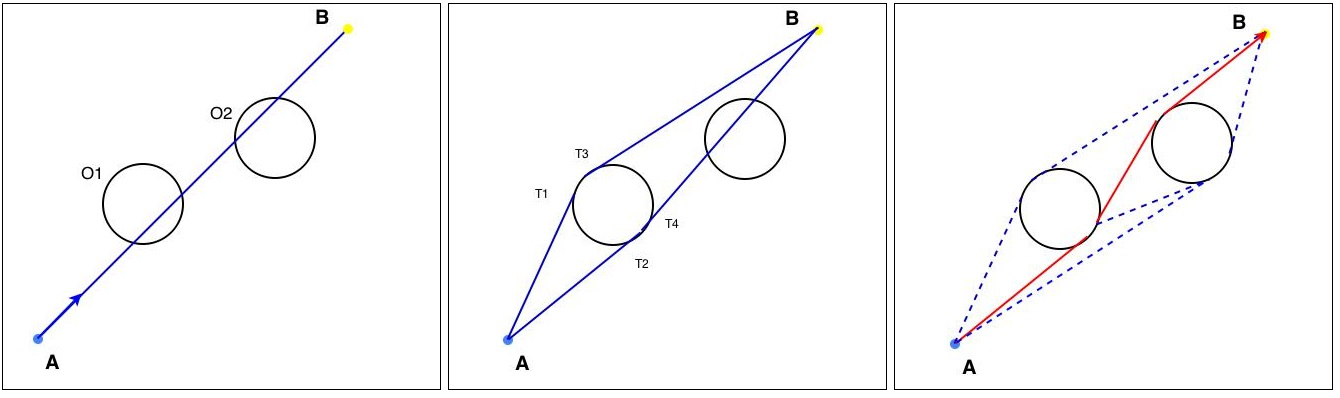
\includegraphics[width=\textwidth,height=5.5cm]{path_paper.jpg}
\caption{(a)Start point A and End Point B hindered by two obstacles (b) Drawing tangents to the first obstacle encountered at $T_{1}$, $T_{2}$, $T_{3}$ and $T_{4}$. (c) Recursively following the same function. Final path as shown in red. }
\end{figure*}


Thus in this case since the polygons are treated as circles, if a common tangent to the two circles intersects a circle then common tangents are drawn to this new circle. This process is repeated until we have the entire visibility graph, connecting the start and end point as shown step by step in Algorithm 1. The function of Visibility Graph is called recursively on each of the edge joining two nodes. Thus the number of points in the graph depends on the number of obstacles present on the field which is usually in 3 and in maximum cases 5 including possible erroneous cases. Then to calculate the final trajectory the least cost is found for a path connecting the start and the end point. The entire algorithm is diagrammatically represented in Fig. 1.\\
Now to find the shortest path between the start and end point its all about finding the shortest cost between them in the Visibility Graph. For this purpose Dijkstra's Algorithm[10] is used as it is asymptotically the fastest known single source shortest path algorithm for arbitrary directed graphs with unbounded non-negative weights. Any other graph search algorithm can also be used in this case. 

\subsection{Orientation Circles}
Joining line between the start and end points is not sufficient to give complete path between the two points. It often is required that the bot face a particular direction once it reaches the destination. In this scenario in particular, the humanoid is required to reach the ball, dribble or kick ball towards the goal posts to simply ensure that it does not shoot in the wrong direction or pass the ball to another player or hit another obstacle. One alternative is to simple reach the final point and then orient itself correctly, which leads to dependency on side walk in a circle. A much efficient solution would be consider the correct orientation in the path itself such that when the bot reaches the final point it finds itself oriented in a correct manner. This can be done by simple addition of dummy obstacles of required radius orthogonal to the facing direction, and choosing the final path intelligently. The diagrammatic representation is as shown in the figure 2. 
\begin{figure}[h]  
\begin{center}  
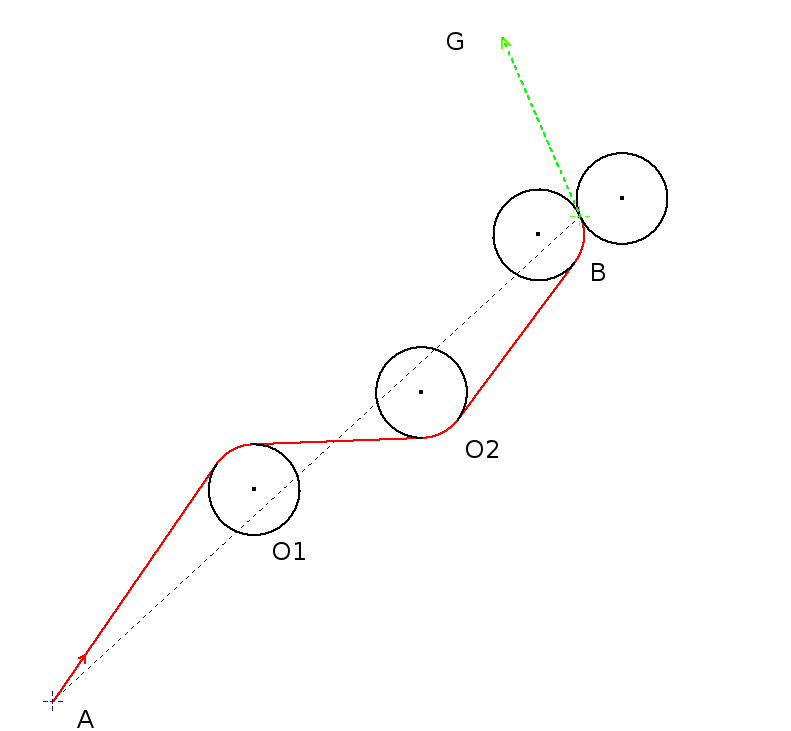
\includegraphics[scale=0.42]{orientation_circle2.JPG}  
\caption{\small \sl Use of orientation circle or dummy obstacles to align the robot correctly. The robot starts from point A, navigates it way around the obstacles $O_1$ and $O_2$, to reach the point B facing the direction G. .\label{fig:orientation}}  
\end{center}  
\end{figure} 
\\
Another use of introduction of dummy obstacles is to start the tracing of the path smoothly. It often happens that the bot is facing a direction and need to start walking at a specified angle to the current gait vector. Since instantaneous turning of the point can prove to be difficulty or time consuming an obstacle can be placed to ensure smooth transition.

\subsection{Edge Cases and Erroneous Inputs}
Since the algorithm is dynamic some cases will arise when the robot, obstacle, ball all are very near, especially when the bot progressively reaching its target. In such cases due to erroneous inputs from the camera, sometimes the bot or end point can be found inside the obstacle itself, making it impossible to draw tangents. Such cases are ignored and since the frame rate is as high as 50 fps these instances do not matter much and are taken care of in the subsequent frames.
\\ 
Other cases include when obstacles intersect. This may be because of the erroneous inputs if obstacles are behind one another or because of the generic assumption that obstacles all have the same radius. This in addition to the fact that obstacles radius is its radius added with the half of radius of the bot itself so that the test subject can easily maneuver between obstacles. To solve this problem any two such intersecting obstacles are treated as one obstacle, by making a best fitting polygon usually an ellipse on top of the obstacles. The algorithm can be now executed normally considering this new ellipse.

\begin{figure}[h]  
\begin{center}  
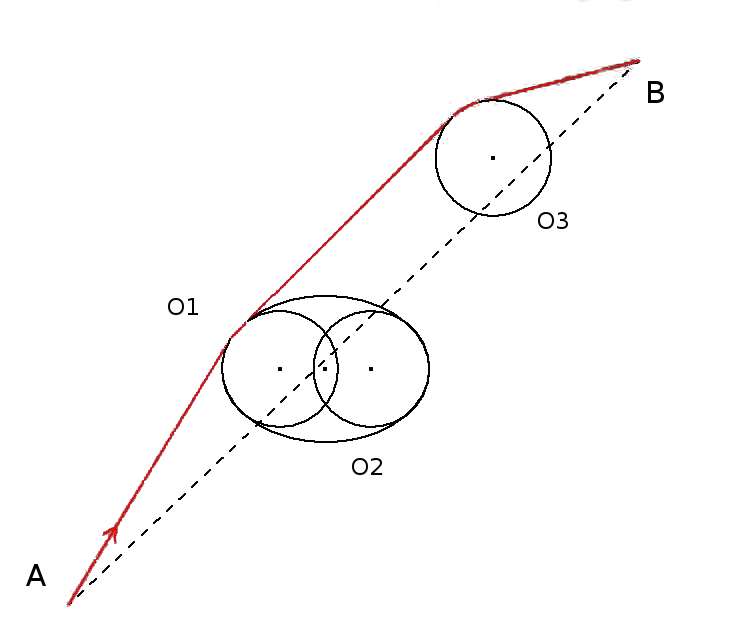
\includegraphics[scale=0.3]{intersection1.JPG}  
\caption{\small \sl Dealing with intersection of obstacles due to erroneous inputs.\label{fig: intersection}}  
\end{center}  
\end{figure}

\subsection{Hierarchical Controller}
The hierarchical motion controller implemented on the humanoid is presented below for providing a clear picture of the step planning interface. 
The placement of the footstep planning interface in the behavioral chain of
events is between the path planning algorithm and the high-level position
controller of the humanoid gait generation module. The
controller is hierarchically structured into three components:
	\begin{enumerate}[A)]
\item Position Control Module
\item Gait Generation Module
\item Inverse Kinematics Module

The salient features of the modules are discussed below:
\end{enumerate}
	\begin{enumerate}[A)]
  \item A high level 3 Dimensional step position S is
  supplied to the gait generation controller. S is defined as:
  	
  	\begin{center}$S \in (Z, Y, \theta)$\end{center}
 where Z and Y are the lateral and sagittal displacements of the
 free leg with respect to the current 2 dimensional projection of the CoM on
  the ground. $\theta$ describes the rotation of the foot with respect
  to the present orientation of the humanoid. 

The limits on acceptable step position values arise from theoretical constraints of the implemented motion generator and the physical constraints of the humanoid. 
In the humanoid under discussion, theoretical limits are placed on the range of attainable step positions which derive from a range of attainable velocities.
The step planning interface is responsible for generating acceptable step positions, and the specific implementation of such an interface is discussed in the next subsection.
  	
  $S$ is presented to the Gait Generation Module as a commanded target position at the end of the step.
  \item Although the step parameter is commanded on the free leg, the final velocity attained after the step is precomputed in order
to present a target velocity for the support leg trajectories. In the humanoid under discussion the support leg operates on 3D LIPM trajectories parameterized by current velocity and target velocity. Therefore the commanded step position is used to compute the final velocity, which is used to generate stable 3D LIPM trajectories. 
  
  The present position in the trajectory is advanced with time at every frame,
  and the new coordinates are forwarded to the Inverse Kinematics (IK) Module.
  \item Joint angles, and the corresponding motor
  positions are calculated by the IK as a solution to the present step
  coordinates presented by the gait generation module at each frame. The motors
  are then instructed to attain these values such that the desired motion can be
  obtained.
\end{enumerate}

The reason for such a hierarchical structure is that it allows changes at each
tier without requiring changes to the other tiers on hierarchy. For instance,
the IK module can be adapted for a humanoid robot with a
different mechanical structure, without having to change the gait generation
module. Similarly, the present gait generation algorithm can be freely changed
for purposes of experimentation without making any changes in the IK module. However, the step planning interface must be designed to generate acceptable step positions and may require changes depending on the gait generation algorithm being used and the mechanical limitations of the humanoid.

\subsection{Step Planning Interface}
The step planning interface decomposes the path into discrete footsteps which result in the robot following the desired trajectory.

The path is first broken down into two components:
\begin{itemize}
  \item Straight Line Path
  \item Circular Path
\end{itemize}

When the designated trajectory is a straight line, the robot accelerates to its maximum velocity and footstep vectors are generated for the maximum step length and velocity until the distance covered by the robot is equivalent to the straight line length. 
 
When the trajectory is circular, the step planning interface generates footstep vectors using the radius of the circle and the separation of the feet. Each step advances the angle turned by the $\theta$ component of the step vector. When the target turning angle is achieved, the robot will have traversed the circular arc with the desired turning radius. It is not possible to have a constant velocity when navigating a circular path, because the steps taken by the foot on the inner side of the circle are shorter than the outer foot. Therefore, the velocity stabilizes by oscillating between two different values. \\ 
The transition between a straight line trajectory to a circular one and vice versa must be handled smoothly since at any frame the new path generated may possess a straight line or a circle. Given the present velocity and step location, the interface must generate stable transition of velocity (acceleration or deceleration) to adapt to the new trajectory. This situation is accommodated by allowing a margin of one or two steps to transition safely to the new trajectory. The inaccuracy introduced by this margin is negligible due to the high step frequency of the robot.

The step planning interface needs to be constrained in some manner to prevent drastic sudden changes in the velocity of the humanoid. Since the robot is presented with an online path planner, the robot may be asked to accomodate changes in path radius at each step.
In this humanoid, the constraints are derived from a reformulation of the standard 3D LIPM equations:

3D Linear Inverted Pendulum Model describes the motion of the Centre of Mass (CoM) in the robot[12]. The motion of support leg is opposite of the CoM, since the support leg behaves as a pivot which moves the CoM of the robot. Therefore the 3D LIPM algorithm can be used to develop a relation between step lengths and CoM velocities. The motion of the robot's supporting leg is defined by the x-variable in the Eq 1. Tc and Ts are constants, Ts being the SSP time of the robot. The initial and final states of the bot (before and after the step) are represented by i and f. Velocity and position are denoted by $v$ and $x$.
\\

\begin{equation}
\left(\begin{array}{c}x_{f}\\\\ v_{f}\end{array}\right)=\left(\begin{array}{cc}\cosh\left(\frac{T_{s}}{T_{c}}\right) & T_{c}\sinh\left(\frac{T_{s}}{T_{c}}\right) \\\\ \frac{\sinh\left(\frac{T_{s}}{T_{c}}\right)}{T_{c}} & \cosh\left(\frac{T_{s}}{T_{c}}\right)\end{array}\right)\left(\begin{array}{c}x_{i}\\\\ v_{i}\end{array}\right)
\end{equation}

Since the step planner only observes discrete footsteps and not any arbitrary moment in time, the $T_{s}$ is treated as the constant end-of-step time, instead of the variable time $t$. During trajectory generation the variable $T_{s}$ is replaced by current step time $t$, which reaches the value $T_{s}$ at the end of the step.

The above equations are reformulated as:
\begin{equation}
x_{f} = A\sinh\left(T_{s}/T_{c} + \phi\right)
\end{equation}
\begin{equation}
v_{f} = A\cosh\left(T_{s}/T_{c} + \phi\right)
\end{equation}
where,
\begin{equation}
 A=v_{i}\sqrt{T_{c}^{2}-\left(\frac{x_{i}}{T_{c}}\right)^{2}}
  \end{equation}
  \begin{equation}
  \phi=\sinh^{-1}\left(\frac{x_{i}}{A}\right)
\end{equation}
 This reformulation represents a loss in generality, since it implicitly
 introduces the assumption that the humanoid only moves forward, and does not
 perform maneuvers such as a back walk. This implementation also introduces
 certain constraints on the maximum and minimum future velocity relative to
 the present velocity. The reformulation is carried out for the purpose of deriving these constraints,
thereby restraining the motion of the humanoid by preventing it from drastic changes in velocity. The standard LIPM equations suffice for changing the humanoid's state from stationary to a moving
initial velocity, and for back walk. Alternatively, these constraints may be forgone in favor of experimentally derived limits on acceleration and deceleration, and the equations which follow below 
represent a theoretically obtainable limit, which need not be observed in the standard LIPM formulation.
\\
The constraints are derived in
 the form of maximum and minimum ratios of initial and final velocity over a single step $\left(v_{f}/v_{i}\right)$.\\
 The constraints are derived to obtain the following range:

 \begin{equation}
 \left(\frac{v_f}{v_d}\right)_{min} =\enspace p - \sqrt{p^2 - 1}
 \end{equation}
 and
 \begin{equation}
 \left(\frac{v_f}{v_d}\right)_{max}=\enspace p
 \end{equation}
 Or,
 \begin{equation}
(v_f)_{min}	    = \left(p - \sqrt{p^2 - 1}\right)v_d
 \end{equation}
 \begin{equation}
 (v_f)_{max}=pv_d
  \end{equation}

  where \begin{equation}
 p=\cosh\left(\frac{T_s}{T_c}\right)
 \end{equation}
It must be noted that the above range is independent of all other earlier states, such as $v_i$ and $y_i$, which means that the range applies to any step considered independently.\\
The footstep positions generated by a given path have been pictorially presented in Fig 4. Each circle indicates where the humanoid will place its foot. It may be observed from the image that the step lengths are considerably less along the circular arcs. This indicates the decreased velocity of the robot when turning. Furthermore, the first two steps on the circle possess a step length which is shorter than the maximum step length, but not equal to the step length of the feet during the circular motion. This indicates the transition from maximum velocity to the circular velocity, with two intermediate steps to smoothen the transition. If the velocity constraints described above were not in place, the circular trajectory would have resulted in an immediate velocity drop, leading to instability. This transition is all the more critical in the scenario where the online path alternately generated a line and a circle, which would result in a sudden transition from maximum velocity to circular velocity, and then back to maximum velocity. The same intermediate steps may be observed whenever the robot exits the circle.
\begin{figure}[h]  
\begin{center}  
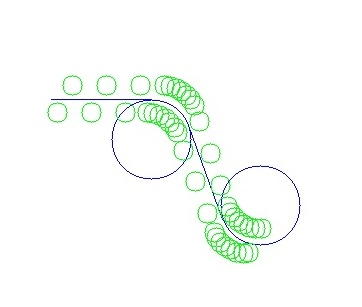
\includegraphics[scale=01.0]{footstep.jpg}  
\caption{\small \sl Footstep locations for the given path.\label{fig:footstep}}  
\end{center}  
\end{figure}

\section{Experiment and Results}
Visibility graph in this case consists of $(4*n+2)$ number of points in the worst case, where $n$ in the number of obstacles intersecting the line joining the start and end point, i.e. coming in the way of the bot to reach the goal position. The visibility graph can be calculated in worst case time of $O(n^2)$. Further more the Dijkstra's has a wost case performance of $O(4n+4n*log(4n))$. Thus this algorithm decreases the number of node points on which a graph search can be applied with ease. \\
\begin{figure}[h]  
\begin{center}  
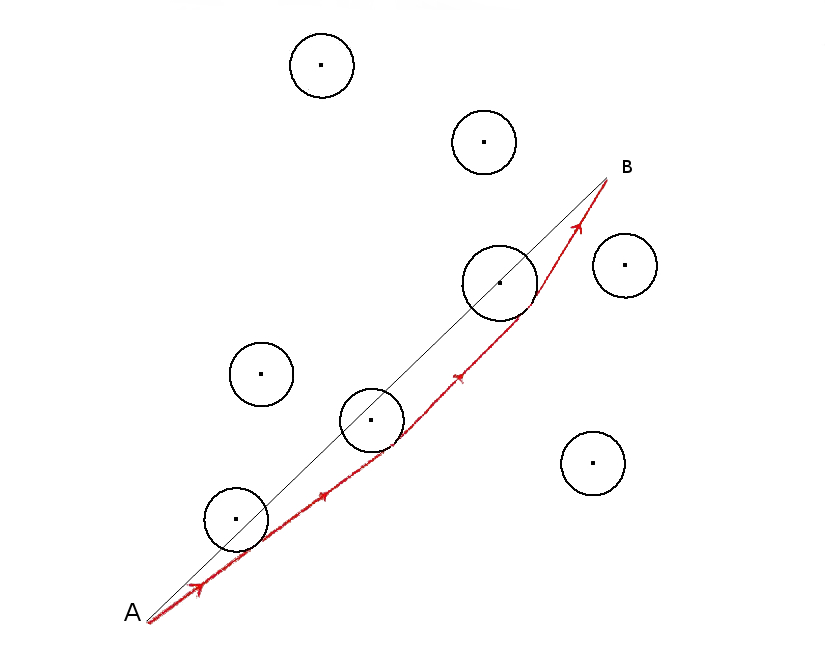
\includegraphics[scale=0.3]{test1.JPG}  
\caption{\small \sl The use of path planning for multiple obstacles. \label{fig:test}}  
\end{center}  
\end{figure}
The footstep planning interface along with the path planning were integrated with the behavior layer of the humanoid for testing purposes. For the experimental setup, two obstacles of radius 15 cm each were placed in the way of the bot and the ball. The bot had to navigate its way around the obstacles and align itself to hit the ball towards the goalposts. Both the scenarios where obstacles were static and dynamic were devised to test the efficacy of the algorithm. The tests were conducted for a total of more than 200 configurations in both cases. The advantages which were very apparent that the bot was able to correct its trajectory when it lost track of the path, due to losing its stability or some mechanical disturbances like friction. In the dynamic scenario some oscillation at a point were observed where the robot has to choose between two equally probable paths. Such edge cases can be easily be solved by either random selection or adjusting the frequency of mapping final path to the gait vector.\\

\begin{figure}[h]  
\begin{center}  
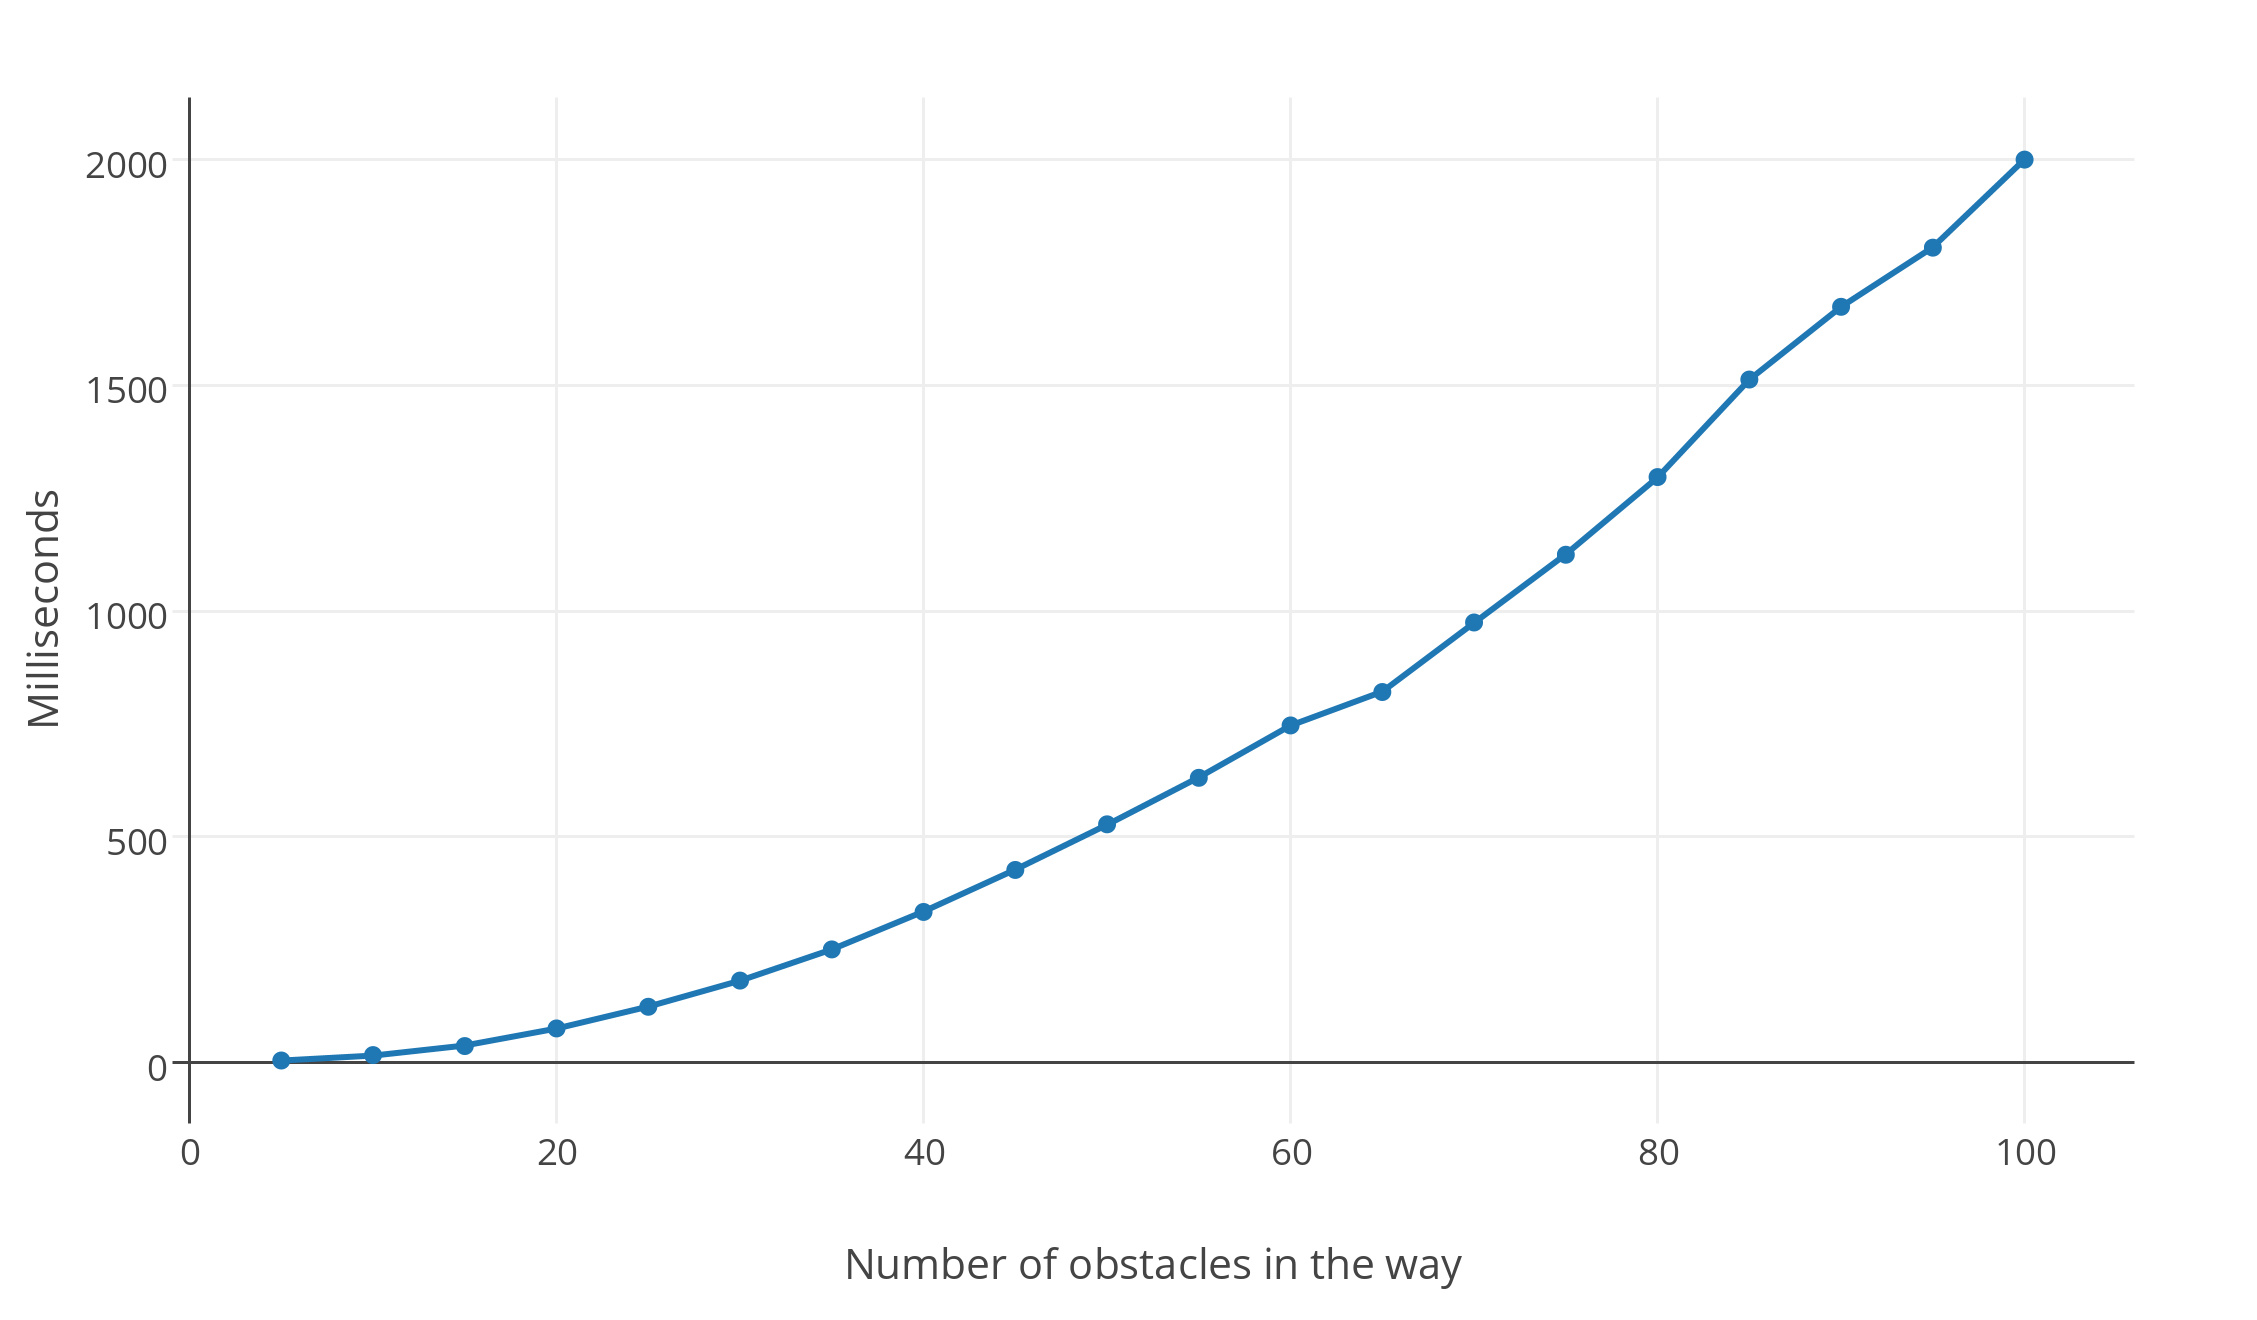
\includegraphics[width=8cm, height = 7cm]{test2.jpg}  
\caption{\small \sl Time dependency of the algorithm on the number of obstacles in the robot's way. \label{fig:test2}}  
\end{center}  
\end{figure}

The number of obstacles particularly in Robocup are small. There can be at a time a maximum of 3 obstacles. The worst case scenario that all three obstacles are in the robot's way, would involve the calculation of shortest path algorithm on a visibility graph consisting of just 14 points. When tested on the actual platform with 3 obstacles the average time taken to calculate was around 4 ms. This time is sufficient to give the entire cognition module a frame rate of 50 fps. Thus at such high frame rates, the dynamic nature of the obstacles is easily taken care of. The noise from the sensors like camera and the deviation of walk are thus handled naturally as a result of this. Fig. 5 shows the results of using the algorithm for an arbitrary configuration that might occur in a technical challenge in Robocup where the bot has to navigate its way and dribble a ball along with it. Testing this algorithm for up to 100 obstacles between the robot and its target gave the results as shown in Fig 6.
 

\section{Comparison}
The algorithm presented here is compared with the other standard planning algorithms in terms of time taken, and no. of operations. The algorithm discussed in this paper is applicable to very specific cases, especially when the size of the obstacle is comparable to that of the robot itself. One of the main advantages of this geometry based planning algorithm is the non dependency on grids. Usually algorithms based on grids computationally expensive or do not have high resolution. The algorithm presented works in a grid less environment and only considers the nodes of interest, instead of analyzing each and every point on the map. Moreover it is not restricted to frame area of any size whatsoever, meaning the obstacles, final position can be located anywhere with reference to the navigating object without any cost to computation.\\
For comparing this algorithm with the other standard ones in the literature we considered the setup of 2 obstacles along the way to the final point as shown in Fig. 7. The results of the comparison are as tabulated in Table 1.\\ 
\begin{center}
    \begin{tabular}{| p{3cm} | l | p{2.5cm} |}
    \hline
    \textbf{Algorithm} & \textbf{Time (ms)} & \textbf{No. of Operations} \\ \hline
    Geometry based & 3.6 & 84  \\ \hline
    $A^{*}$,  & 5 & 243  \\ \hline
    Breadth First Search & 13  & 1013 \\
    \hline
    Best First Search & 5  & 95 \\ \hline
    Dijkstra & 18  & 1161 \\ \hline
    Artificial Potential Mapping & 6 & 57\\ \hline
    \end{tabular}
\end{center}
\begin{center}
\small{Table 1: Comparison of Various Path Planning Algorithms\\}
\end{center}

\begin{figure}[h]  
\begin{center}  
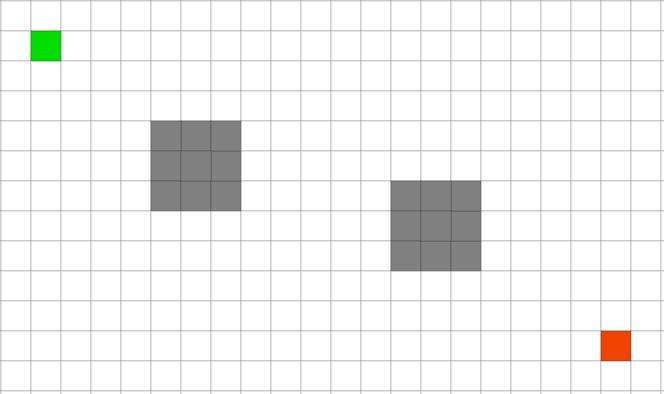
\includegraphics[scale=0.4]{testbed.jpg}  
\caption{\small \sl Testing variables for various algorithms above.\label{fig:test3}}  
\end{center}  
\end{figure}


\section{Conclusion}
We have presented an unique way for path planning which is best suitable to the case when the obstacles size is comparable to the robots. In such cases we can take advantage of the robots shape which can be approximated to simple circles to find the best way possible around them using simple geometry. This way we reduce the number of node points on which a graph search can be applied. This reduces the computation time significantly thus giving better frame rates for the execution of code on an on board processor. This way the dynamic nature of the robot soccer games can easily be taken care of along with any noise from the sensors and deviation from the walk. This is then ported to the 3D-LIPM walking pattern generator to adjust the footsteps, gait in such a way that the robot is stable while following the given path. 
\\




\section{Acknowledgment}


The authors would like to thank the Department of Electronics and Information Technology, Government of India who funded the research project. The experiments were carried out at Centre for Robotics and Intelligent Systems, BITS Pilani.

\addtolength{\textheight}{-12cm}  

\begin{thebibliography}{99}
\bibitem{Footstep 1}J. Chestnutt, M. Lau, G. Cheung, J. Kuffner, J. K. Hodgins, and
T. Kanade, "Footstep planning for the Honda ASIMO humanoid", in
\emph{Proc. of the IEEE Int. Conf. on Robotics and Automation} (ICRA?05),
April 2005.
\bibitem{Footstep 2} Y. Ayaz, T. Owa, T. Tsujita, A. Konno, K. Munawar, and M. Uchiyama,
"Footstep planning for humanoid robots among obstacles of various
types", in \emph{Proc. IEEE-RAS Conf. Humanoid Robots}, Dec. 2009, pp. 361-366.
\bibitem{ourima} Lina Ourima, "Fast Geometric Path Planning for the Small Size Robocup League", Friei Universitat Berlin, June 2004
\bibitem{a*} Maren Bennewitz and Wolfram Burgard, Finding Solvable Priority Schemes for Decoupled Path Planning Techniques for Teams of Mobile Robots, \emph{PROCEEDINGS OF THE 9TH INTERNATIONAL SYMPOSIUM ON INTELLIGENT ROBOTIC SYSTEMS}, 2001
\bibitem{5} Ricarda Steffens et. al., Multiresolution Path Planning in Dynamic Environments for the Standard Platform League, \emph{Proceedings of the 5th Workshop on Humanoid Soccer Robots @ Humanoids 2010}, Dec. 2010
\bibitem{6} Oussama Khatib, Real-time obstacle avoidance
for manipulators and mobile robots," \emph{Proceedings
of the 1985 IEEE International Conference
on Robotics and Automation}, St. Louis, MO, May
1985
\bibitem{7} Sven Koenig et. al., D* Lite, American Association for Artificial Intelligence, 2002
\bibitem{8} J. Chestnutt, J. Kuffner, K. Nishiwaki, and S. Kagami, ?Planning biped
navigation strategies in complex environments,? in \emph{Proc. of the IEEERAS/RSJ
Int. Conf. on Humanoid Robots (Humanoids?03)}, Munich,
Germany, October 2003.
\bibitem{9} Andreas Schmitz, Marcell Missura, and Sven Behnke, "Real-time trajectory generation
by offline footstep planning for a humanoid soccer robot",  In \emph{Proceedings of
15th RoboCup International Symposium, Istanbul}, 2011.
\bibitem{10} Huijuan Wang  et. al., Application of Dijkstra algorithm in robot
path-planning, 
\bibitem{11} S. Kajita, F. Kanehiro, K. Kaneko, K. Yokoi and H. Hirukawa, "The 3D linear inverted
pendulum model: a simple modeling for a biped walking pattern generation", \emph{In
IROS}, 2001, Vol. 1, pp. 239-246
\bibitem{12} H. Alt and E. Welzi, Visibility Graphs and Obstacle Avoiding shortest paths, \emph{Zeitschrift für Operations Research},1998


\end{thebibliography}




\end{document}
